\documentclass[onecolumn]{revtex4}
\usepackage{fancyhdr}
\usepackage{html}
\usepackage{graphicx}
\usepackage{url}
\begin{document}
\title{Equilibrium parameters of the PAW atomic data}
\date{\today}
\author{\textsc{Abinit}}
\affiliation{\url{http://wwww.abinit.org}}
\begin{abstract}
The present results have been obtained through the use of the ABINIT code, 
a common project of the Universit\'e Catholique de Louvain, Corning
Incorporated, and other contributors~\cite{ABINIT,ABINITbis}, in the framework of the Projector augmented-wave (PAW)
method introduced by Peter Bl\"ochl in 1994~\cite{Blochl_PRB50_1994}. 


The atomic data are generated using the
PAW atomic data generator (ATOMPAW) written by N. Holzwarth~\cite{Holzwarth_PRB55_1997,Holzwarth_PRB57_1998,Tackett_CPC135_2001}.


Versions of the ABINIT and ATOMPAW codes are x.y.z and a.b.c.
\end{abstract}
\maketitle
\section{PURE MATERIALS: Bulk and dimer properties}
\newpage
\paragraph*{\bf{PURE/OUTPUT/001-H}}
\begin{center}
\begin{tabular}{lc}
\hline
Index & Atomic data file \\
\hline
1 & \verb?001-H/GGA-ATOMPAW-fbrc1/H.GGA-PBE-paw.abinit?\\
2 & \verb?001-H/GGA-ATOMPAW-fbrc2/H.GGA-PBE-paw.abinit?\\
3 & \verb?001-H/LDA-ATOMPAW-fbrc1/H.LDA-PW-paw.abinit?\\
4 & \verb?001-H/LDA-ATOMPAW-fbrc2/H.LDA-PW-paw.abinit?\\
5 & \verb?001-H/H-GGA-hard-uspp/H-GGA-hard-uspp.paw?\\
6 & \verb?001-H/H-GGA-uspp/H-GGA-uspp.paw?\\
7 & \verb?001-H/H-LDA-hard-uspp/H-LDA-hard-uspp.paw?\\
8 & \verb?001-H/H-LDA-uspp/H-LDA-uspp.paw?\\
\hline
\end{tabular}
\end{center}
\begin{center}
\begin{tabular}{lccccc}
\hline
\hline
\bf{fcc}&$V_0$ (\AA$^3$/atom)&$E_{\rm coh}$ (eV/atom)&$B_0$ (Gpa)&$B_0^{'}$& \\
\hline
1.fcc.out (20,40)& 2.973 &-1.029 & 105.0 & 3.5 & \\ 
2.fcc.out (14,28)& 3.023 &-1.019 & 107.8 & 2.7 & \\ 
3.fcc.out (20,40)& 2.915 &-1.559 & 112.1 & 3.4 & \\ 
4.fcc.out (12,24)& 2.970 &-1.548 & 112.9 & 3.9 & \\ 
5.fcc.out (12,24)& 2.997 &-1.028 & 104.6 & 3.6 & \\ 
6.fcc.out (10,20)& 2.968 &-1.033 & 104.5 & 2.7 & \\ 
7.fcc.out (12,24)& 2.937 &-0.990 & 112.8 & 3.5 & \\ 
8.fcc.out (10,20)& 2.912 &-0.995 & 110.9 & 2.7 & \\ 
\hline
\hline
\bf{dimer}&\multicolumn{2}{c}{$E_{\rm bind}$ (eV/dimer)}&\multicolumn{3}{c}{$d_{\rm eq}$ (\AA)} \\
\hline
1.dimer.out (20,40)&\multicolumn{2}{c}{-4.506}&\multicolumn{2}{c}{0.756} \\ 
2.dimer.out (14,28)&\multicolumn{2}{c}{-4.481}&\multicolumn{2}{c}{0.757} \\ 
3.dimer.out (20,40)&\multicolumn{2}{c}{-4.878}&\multicolumn{2}{c}{0.770} \\ 
4.dimer.out (12,24)&\multicolumn{2}{c}{-4.849}&\multicolumn{2}{c}{0.771} \\ 
5.dimer.out (12,24)&\multicolumn{2}{c}{-4.508}&\multicolumn{2}{c}{0.753} \\ 
6.dimer.out (10,20)&\multicolumn{2}{c}{-4.509}&\multicolumn{2}{c}{0.758} \\ 
7.dimer.out (12,24)&\multicolumn{2}{c}{-1.1354814009}&\multicolumn{2}{c}{0.76818947628} \\ 
8.dimer.out (10,20)&\multicolumn{2}{c}{-1.1354387619}&\multicolumn{2}{c}{0.77280044347} \\ 
NC GGA dimer~\cite{Tutorial2_ABINIT} & \multicolumn{2}{c}{-4.482} & \multicolumn{2}{c}{0.754} \\ %001-H
NC LDA dimer~\cite{Tutorial2_ABINIT} & \multicolumn{2}{c}{-4.833} & \multicolumn{2}{c}{0.769} \\ %001-H
PAW LDA dimer~\cite{Blochl_PRB50_1994} & \multicolumn{2}{c}{-4.62} & \multicolumn{2}{c}{0.773} \\ %001-H
PAW GGA dimer~\cite{Kresse_SS459_2000} & \multicolumn{2}{c}{-4.58} & \multicolumn{2}{c}{0.750} \\ %001-H
PAW GGA dimer~\cite{Jiang_PRB70_2004} & \multicolumn{2}{c}{-4.54} & \multicolumn{2}{c}{0.750} \\ %001-H
Experiment dimer~\cite{Huber_1979} & \multicolumn{2}{c}{-4.75} & \multicolumn{2}{c}{0.741} \\ %001-H
\hline
\hline
\end{tabular}
\end{center}
\begin{figure}[h] 
\centering 
\includegraphics[height=0.7\textwidth,width=0.5\textwidth,angle=-90]{PURE/OUTPUT/001-H/ecut.eps}
\end{figure}
\begin{figure}[h] 
\centering 
\includegraphics[height=0.7\textwidth,width=0.5\textwidth,angle=-90]{PURE/OUTPUT/001-H/fcc.eps}
\end{figure}
\newpage
\paragraph*{\bf{PURE/OUTPUT/005-B}}
\begin{center}
\begin{tabular}{lc}
\hline
Index & Atomic data file \\
\hline
1 & \verb?005-B/B-GGA-atompaw/B.GGA-PBE-paw.abinit?\\
2 & \verb?005-B/B-GGA-hard-atompaw/B.GGA-PBE-paw.abinit?\\
3 & \verb?005-B/B-LDA-atompaw/B.LDA-PW-paw.abinit?\\
4 & \verb?005-B/B-LDA-hard-atompaw/B.LDA-PW-paw.abinit?\\
\hline
\end{tabular}
\end{center}
\begin{center}
\begin{tabular}{lccccc}
\hline
\hline
\bf{fcc}&$V_0$ (\AA$^3$/atom)&$E_{\rm coh}$ (eV/atom)&$B_0$ (Gpa)&$B_0^{'}$& \\
\hline
1.fcc.out (12,24)& 5.892 &-4.869 & 263.2 & 4.2 & \\ 
2.fcc.out (24,48)& 5.882 &-4.859 & 272.6 & 3.9 & \\ 
3.fcc.out (12,24)& 5.696 &-5.777 & 287.2 & 4.2 & \\ 
4.fcc.out (22,44)& 5.695 &-5.776 & 295.6 & 4.3 & \\ 
\hline
\hline
\bf{dimer}&\multicolumn{2}{c}{$E_{\rm bind}$ (eV/dimer)}&\multicolumn{3}{c}{$d_{\rm eq}$ (\AA)} \\
\hline
1.dimer.out (12,24)&\multicolumn{2}{c}{-3.351}&\multicolumn{2}{c}{1.619} \\ 
2.dimer.out (24,48)&\multicolumn{2}{c}{-3.338}&\multicolumn{2}{c}{1.619} \\ 
3.dimer.out (12,24)&\multicolumn{2}{c}{-3.852}&\multicolumn{2}{c}{1.605} \\ 
4.dimer.out (22,44)&\multicolumn{2}{c}{-3.844}&\multicolumn{2}{c}{1.606} \\ 
PAW LDA dimer~\cite{Blochl_PRB50_1994} & \multicolumn{2}{c}{-3.78} & \multicolumn{2}{c}{1.603} \\ %005-B
\hline
\hline
\end{tabular}
\end{center}
\begin{figure}[h] 
\centering 
\includegraphics[height=0.7\textwidth,width=0.5\textwidth,angle=-90]{PURE/OUTPUT/005-B/ecut.eps}
\end{figure}
\begin{figure}[h] 
\centering 
\includegraphics[height=0.7\textwidth,width=0.5\textwidth,angle=-90]{PURE/OUTPUT/005-B/fcc.eps}
\end{figure}
\newpage
\paragraph*{\bf{PURE/OUTPUT/006-C}}
\begin{center}
\begin{tabular}{lc}
\hline
Index & Atomic data file \\
\hline
1 & \verb?006-C/GGA-ATOMPAW-fbrc1/C.GGA-PBE-paw.abinit?\\
2 & \verb?006-C/GGA-ATOMPAW-fbrc2/C.GGA-PBE-paw.abinit?\\
3 & \verb?006-C/LDA-ATOMPAW-fbrc1/C.LDA-PW-paw.abinit?\\
4 & \verb?006-C/LDA-ATOMPAW-fbrc2/C.LDA-PW-paw.abinit?\\
5 & \verb?006-C/C-GGA-hard-uspp/C-GGA-hard.paw?\\
6 & \verb?006-C/C-GGA-uspp/C-GGA-uspp.paw?\\
7 & \verb?006-C/C-LDA-hard-uspp/C-LDA-hard-uspp.paw?\\
8 & \verb?006-C/C-LDA-uspp/C-LDA-uspp.paw?\\
\hline
\end{tabular}
\end{center}
\begin{center}
\begin{tabular}{lccccc}
\hline
\hline
\bf{diamond}&$V_0$ (\AA$^3$/atom)&$E_{\rm coh}$ (eV/atom)&$B_0$ (Gpa)&$B_0^{'}$& \\
\hline
1.diamond.out (26,52)& 5.703 &-7.698 & 433.6 & 3.8 & \\ 
2.diamond.out (16,32)& 5.726 &-7.711 & 431.8 & 3.6 & \\ 
3.diamond.out (28,56)& 5.514 &-8.928 & 467.1 & 3.7 & \\ 
4.diamond.out (16,32)& 5.537 &-8.913 & 465.7 & 3.6 & \\ 
5.diamond.out (14,28)& 5.727 &-7.697 & 434.5 & 3.6 & \\ 
6.diamond.out (12,24)& 5.705 &-7.749 & 436.7 & 3.8 & \\ 
7.diamond.out (14,28)& 5.542 &-8.220 & 467.0 & 3.6 & \\ 
8.diamond.out (12,24)& 5.522 &-8.337 & 470.5 & 3.7 & \\ 
PAW LDA diamond~\cite{Kresse_PRB59_1999} & 5.522  & - & 460 & - \\ %006-C
PAW LDA diamond~\cite{Holzwarth_PRB55_1997} & 5.545 & - & 460 & - \\ %006-C
LAPW LDA diamond~\cite{Holzwarth_PRB55_1997} & 5.545 & - & 470 & - \\ %006-C
Experiment diamond~\cite{Kittel_1996} & 5.640 & -7.37 & 443 & - \\ %006-C
\hline
\hline
\end{tabular}
\end{center}
\begin{figure}[h] 
\centering 
\includegraphics[height=0.7\textwidth,width=0.5\textwidth,angle=-90]{PURE/OUTPUT/006-C/ecut.eps}
\end{figure}
\begin{figure}[h] 
\centering 
\includegraphics[height=0.7\textwidth,width=0.5\textwidth,angle=-90]{PURE/OUTPUT/006-C/diamond.eps}
\end{figure}
\newpage
\paragraph*{\bf{PURE/OUTPUT/007-N}}
\begin{center}
\begin{tabular}{lc}
\hline
Index & Atomic data file \\
\hline
1 & \verb?007-N/N-GGA-hard-uspp/N-GGA-hard-uspp.paw?\\
2 & \verb?007-N/N-LDA-hard-uspp/N-LDA-hard-uspp.paw?\\
\hline
\end{tabular}
\end{center}
\begin{center}
\begin{tabular}{lccccc}
\hline
\hline
\bf{fcc}&$V_0$ (\AA$^3$/atom)&$E_{\rm coh}$ (eV/atom)&$B_0$ (Gpa)&$B_0^{'}$& \\
\hline
1.fcc.out (14,28)& 7.538 &-0.790 & 194.1 & 4.5 & \\ 
2.fcc.out (14,28)& 7.052 &-1.046 & 241.4 & 4.4 & \\ 
\hline
\hline
\bf{dimer}&\multicolumn{2}{c}{$E_{\rm bind}$ (eV/dimer)}&\multicolumn{3}{c}{$d_{\rm eq}$ (\AA)} \\
\hline
1.dimer.out (14,28)&\multicolumn{2}{c}{-10.410}&\multicolumn{2}{c}{1.111} \\ 
PAW GGA dimer~\cite{Paier_JCP122_2005} & \multicolumn{2}{c}{-10.568} & \multicolumn{2}{c}{-} \\ %007-N
Experiment dimer~\cite{Paier_JCP122_2005} & \multicolumn{2}{c}{-9.844} & \multicolumn{2}{c}{-} \\ %007-N
\hline
\hline
\end{tabular}
\end{center}
\begin{figure}[h] 
\centering 
\includegraphics[height=0.7\textwidth,width=0.5\textwidth,angle=-90]{PURE/OUTPUT/007-N/ecut.eps}
\end{figure}
\begin{figure}[h] 
\centering 
\includegraphics[height=0.7\textwidth,width=0.5\textwidth,angle=-90]{PURE/OUTPUT/007-N/fcc.eps}
\end{figure}
\newpage
\paragraph*{\bf{PURE/OUTPUT/008-O}}
\begin{center}
\begin{tabular}{lc}
\hline
Index & Atomic data file \\
\hline
1 & \verb?008-O/GGA-ATOMPAW-fbrc1/O.GGA-PBE-paw.abinit?\\
2 & \verb?008-O/GGA-ATOMPAW-fbrc2/O.GGA-PBE-paw.abinit?\\
3 & \verb?008-O/GGA-ATOMPAW-fbrso/O.GGA-PBE-paw.abinit?\\
4 & \verb?008-O/LDA-ATOMPAW-fbrc1/O.LDA-PW-paw.abinit?\\
5 & \verb?008-O/LDA-ATOMPAW-fbrc2/O.LDA-PW-paw.abinit?\\
6 & \verb?008-O/LDA-ATOMPAW-fbrso/O.LDA-PW-paw.abinit?\\
7 & \verb?008-O/O-GGA-hard-uspp/O-GGA-hard-uspp.paw?\\
8 & \verb?008-O/O-LDA-hard-uspp/O-LDA-hard-uspp.paw?\\
\hline
\end{tabular}
\end{center}
\begin{center}
\begin{tabular}{lccccc}
\hline
\hline
\bf{fcc}&$V_0$ (\AA$^3$/atom)&$E_{\rm coh}$ (eV/atom)&$B_0$ (Gpa)&$B_0^{'}$& \\
\hline
1.fcc.out (32,64)& 7.988 &-0.408 & 144.2 & 4.6 & \\ 
2.fcc.out (18,36)& 8.054 &-0.477 & 139.7 & 4.6 & \\ 
3.fcc.out (36,72)& 8.017 &-0.451 & 141.6 & 4.8 & \\ 
4.fcc.out (32,64)& 7.206 &-1.529 & 201.3 & 4.6 & \\ 
5.fcc.out (18,36)& 7.258 &-1.506 & 195.8 & 4.6 & \\ 
6.fcc.out (38,76)& 7.235 &-1.781 & 215.2 & 5.3 & \\ 
7.fcc.out (16,32)& 7.991 &-0.339 & 142.6 & 4.9 & \\ 
8.fcc.out (16,32)& 7.223 &-0.273 & 202.8 & 4.9 & \\ 
\hline
\hline
\bf{dimer}&\multicolumn{2}{c}{$E_{\rm bind}$ (eV/dimer)}&\multicolumn{3}{c}{$d_{\rm eq}$ (\AA)} \\
\hline
1.dimer.out (32,64)&\multicolumn{2}{c}{-6.195}&\multicolumn{2}{c}{1.222} \\ 
2.dimer.out (18,36)&\multicolumn{2}{c}{-5.957}&\multicolumn{2}{c}{1.255} \\ 
3.dimer.out (36,72)&\multicolumn{2}{c}{-6.308}&\multicolumn{2}{c}{1.224} \\ 
4.dimer.out (32,64)&\multicolumn{2}{c}{-7.494}&\multicolumn{2}{c}{1.209} \\ 
5.dimer.out (18,36)&\multicolumn{2}{c}{-7.066}&\multicolumn{2}{c}{1.242} \\ 
6.dimer.out (38,76)&\multicolumn{2}{c}{-7.622}&\multicolumn{2}{c}{1.227} \\ 
7.dimer.out (16,32)&\multicolumn{2}{c}{-5.981}&\multicolumn{2}{c}{1.228} \\ 
PAW GGA dimer~\cite{Paier_JCP122_2005} & \multicolumn{2}{c}{-6.214} & \multicolumn{2}{c}{-} \\ %008-O
PAW LDA dimer~\cite{Blochl_PRB50_1994} & \multicolumn{2}{c}{-7.33} & \multicolumn{2}{c}{1.228} \\ %008-O
Experiment dimer~\cite{Paier_JCP122_2005} & \multicolumn{2}{c}{-5.116} & \multicolumn{2}{c}{-} \\ %008-O
\hline
\hline
\end{tabular}
\end{center}
\begin{figure}[h] 
\centering 
\includegraphics[height=0.7\textwidth,width=0.5\textwidth,angle=-90]{PURE/OUTPUT/008-O/ecut.eps}
\end{figure}
\begin{figure}[h] 
\centering 
\includegraphics[height=0.7\textwidth,width=0.5\textwidth,angle=-90]{PURE/OUTPUT/008-O/fcc.eps}
\end{figure}
\newpage
\paragraph*{\bf{PURE/OUTPUT/022-Ti}}
\begin{center}
\begin{tabular}{lc}
\hline
Index & Atomic data file \\
\hline
1 & \verb?022-Ti/GGA-ATOMPAW-nh/Ti.GGA-PBE-paw.abinit?\\
2 & \verb?022-Ti/LDA-ATOMPAW-nh/Ti.LDA-PW-paw.abinit?\\
3 & \verb?022-Ti/Ti-GGA-uspp/Ti-GGA-uspp.paw?\\
4 & \verb?022-Ti/Ti-LDA-uspp/Ti-LDA-uspp.paw?\\
\hline
\end{tabular}
\end{center}
\begin{center}
\begin{tabular}{lccccc}
\hline
\hline
\bf{fcc}&$V_0$ (\AA$^3$/atom)&$E_{\rm coh}$ (eV/atom)&$B_0$ (Gpa)&$B_0^{'}$& \\
\hline
1.fcc.out (14,28)& 17.539 &-5.404 & 105.5 & 3.4 & \\ 
2.fcc.out (14,28)& 16.169 &-6.477 & 119.5 & 3.4 & \\ 
3.fcc.out (12,24)& 17.403 &-5.517 & 108.0 & 3.3 & \\ 
4.fcc.out (12,24)& 15.965 &-7.614 & 123.5 & 3.4 & \\ 
LAPW GGA fcc~\cite{Aguayo_PRB65_2002} & 17.4 & - & 107 & - \\ %022-Ti
\hline
\hline
\bf{hcp}&$V_0$ (\AA$^3$/atom)&$E_{\rm coh}$ (eV/atom)&$B_0$ (Gpa)&$B_0^{'}$&c/a \\
&\multicolumn{4}{c}{$\underbrace{\mbox{With an ideal ratio } c/a=\sqrt{8/3}=1.633}_{}$} \\
\hline
1.hcp.out (14,28)& 17.544 &-5.450 & 109.3 & 3.5 & 1.599  \\ 
2.hcp.out (14,28)& 16.235 &-6.516 & 123.6 & 3.5 & 1.618  \\ 
3.hcp.out (12,24)& 17.392 &-5.563 & 111.8 & 3.4 & 1.596  \\ 
4.hcp.out (12,24)& 16.014 &-7.657 & 127.6 & 3.5 & 1.607  \\ 
LAPW GGA hcp~\cite{Aguayo_PRB65_2002} & 17.4 & - & 112 & - & - \\ %022-Ti
PAW GGA hcp~\cite{Jahnatek_PRB71_2005} & 17.049 & - & 118 & - & 1.583 \\ %022-Ti
Experiment hcp~\cite{Simmons_1971} & 17.651 & - & 107 & - & 1.587 \\ %022-Ti
\hline
\hline
\end{tabular}
\end{center}
\begin{figure}[h] 
\centering 
\includegraphics[height=0.7\textwidth,width=0.5\textwidth,angle=-90]{PURE/OUTPUT/022-Ti/ecut.eps}
\end{figure}
\begin{figure}[h] 
\centering 
\includegraphics[height=0.7\textwidth,width=0.5\textwidth,angle=-90]{PURE/OUTPUT/022-Ti/fcc.eps}
\end{figure}
\begin{figure}[h] 
\centering 
\includegraphics[height=0.7\textwidth,width=0.5\textwidth,angle=-90]{PURE/OUTPUT/022-Ti/hcp.eps}
\end{figure}
\newpage
\paragraph*{\bf{PURE/OUTPUT/026-Fe}}
\begin{center}
\begin{tabular}{lc}
\hline
Index & Atomic data file \\
\hline
1 & \verb?026-Fe/Fe-GGA-atompaw/Fe.GGA-PBE-paw.abinit?\\
2 & \verb?026-Fe/Fe-GGA-sp_semicore-atompaw/Fe.GGA-PBE-paw.abinit?\\
3 & \verb?026-Fe/Fe-LDA-atompaw/Fe.LDA-PW-paw.abinit?\\
4 & \verb?026-Fe/Fe-LDA-sp_semicore-atompaw/Fe.LDA-PW-paw.abinit?\\
\hline
\end{tabular}
\end{center}
\begin{center}
\begin{tabular}{lccccc}
\hline
\hline
\bf{fcc}&$V_0$ (\AA$^3$/atom)&$E_{\rm coh}$ (eV/atom)&$B_0$ (Gpa)&$B_0^{'}$& \\
\hline
1.fcc.out (18,36)& 10.334 &-167.121 & 280.3 & 4.9 & \\ 
2.fcc.out (16,32)& 10.310 &-4.905 & 285.7 & 4.7 & \\ 
3.fcc.out (18,36)& 9.572 & 2776.228 & 349.3 & 4.9 & \\ 
4.fcc.out (14,28)& 9.644 &-6.500 & 345.1 & 4.7 & \\ 
LAPW LDA fcc~\cite{Stixrude_PRB50_1994} & 9.641 & - & 340 & 4.4 \\ %026-Fe
LAPW GGA fcc~\cite{Stixrude_PRB50_1994} & 10.272 & - & 288 & 4.4 \\ %026-Fe
\hline
\hline
\bf{bcc}&$V_0$ (\AA$^3$/atom)&$E_{\rm coh}$ (eV/atom)&$B_0$ (Gpa)&$B_0^{'}$& \\
\hline
1.bcc.out (18,36)& 11.457 &-452.375 & 189.6 & 5.7 & \\ 
2.bcc.out (16,32)& 11.385 &-5.060 & 201.6 & 5.3 & \\ 
3.bcc.out (18,36)& 10.402 & 2776.296 & 233.3 & 3.6 & \\ 
4.bcc.out (14,28)& 10.472 &-6.438 & 239.3 & 3.7 & \\ 
PAW LDA bcc~\cite{Kresse_PRB59_1999} & 10.398 & - & 247 & - \\ %026-Fe
PAW GGA bcc~\cite{Kresse_PRB59_1999} & 11.333 & - & 174 & - \\ %026-Fe
LAPW LDA bcc~\cite{Stixrude_PRB50_1994} & 10.481 & - & 245 & 4.6 \\ %026-Fe
LAPW GGA bcc~\cite{Stixrude_PRB50_1994} & 11.386 & - & 189 & 4.9 \\ %026-Fe
LAPW GGA bcc~\cite{Jing_PRB69_2003} & 11.820 & - & - & - \\ %026-Fe
Experiment bcc~\cite{Stixrude_PRB50_1994} & 11.782 & - & 172 & 4.9 \\ %026-Fe
Experiment bcc~\cite{Gong_PRB69_2004} & 11.776 & -4.29 & 173 & - \\ %026-Fe
\hline
\hline
\end{tabular}
\end{center}
\begin{figure}[h] 
\centering 
\includegraphics[height=0.7\textwidth,width=0.5\textwidth,angle=-90]{PURE/OUTPUT/026-Fe/ecut.eps}
\end{figure}
\begin{figure}[h] 
\centering 
\includegraphics[height=0.7\textwidth,width=0.5\textwidth,angle=-90]{PURE/OUTPUT/026-Fe/fcc.eps}
\end{figure}
\begin{figure}[h] 
\centering 
\includegraphics[height=0.7\textwidth,width=0.5\textwidth,angle=-90]{PURE/OUTPUT/026-Fe/bcc.eps}
\end{figure}
\newpage
\paragraph*{\bf{PURE/OUTPUT/027-Co}}
\begin{center}
\begin{tabular}{lc}
\hline
Index & Atomic data file \\
\hline
1 & \verb?027-Co/Co-GGA-atompaw/Co.GGA-PBE-paw.abinit?\\
2 & \verb?027-Co/Co-GGA-sp_semicore-atompaw/Co.GGA-PBE-paw.abinit?\\
3 & \verb?027-Co/Co-GGA-sp_semicore-atompaw/Co.gga.semicore.atompaw?\\
4 & \verb?027-Co/Co-LDA-atompaw/Ni.LDA-PW-paw.abinit?\\
5 & \verb?027-Co/Co-LDA-sp_semicore-atompaw/Co.LDA-PW-paw.abinit?\\
6 & \verb?027-Co/Co-LDA-sp_semicore-atompaw/Co.lda.semicore.atompaw?\\
\hline
\end{tabular}
\end{center}
\begin{center}
\begin{tabular}{lccccc}
\hline
\hline
\end{tabular}
\end{center}
\begin{figure}[h] 
\centering 
\includegraphics[height=0.7\textwidth,width=0.5\textwidth,angle=-90]{PURE/OUTPUT/027-Co/ecut.eps}
\end{figure}
\newpage
\paragraph*{\bf{PURE/OUTPUT/028-Ni}}
\begin{center}
\begin{tabular}{lc}
\hline
Index & Atomic data file \\
\hline
1 & \verb?028-Ni/Ni-GGA-atompaw/Ni.GGA-PBE-paw.abinit?\\
2 & \verb?028-Ni/Ni-GGA-p_semicore-atompaw/Ni.GGA-PBE-paw.abinit?\\
3 & \verb?028-Ni/Ni-GGA-uspp/Ni.uspp.gga.paw?\\
4 & \verb?028-Ni/Ni-LDA-atompaw/Ni.LDA-PW-paw.abinit?\\
5 & \verb?028-Ni/Ni-LDA-p_semicore-atompaw/Ni.LDA-PW-paw.abinit?\\
6 & \verb?028-Ni/Ni-LDA-uspp/Ni.uspp.lda.paw?\\
\hline
\end{tabular}
\end{center}
\begin{center}
\begin{tabular}{lccccc}
\hline
\hline
\end{tabular}
\end{center}
\begin{figure}[h] 
\centering 
\includegraphics[height=0.7\textwidth,width=0.5\textwidth,angle=-90]{PURE/OUTPUT/028-Ni/ecut.eps}
\end{figure}
\newpage
\paragraph*{\bf{PURE/OUTPUT/030-Zn}}
\begin{center}
\begin{tabular}{lc}
\hline
Index & Atomic data file \\
\hline
1 & \verb?030-Zn/Zn-GGA-atompaw/Zn.GGA-PBE-paw.abinit?\\
2 & \verb?030-Zn/Zn-GGA-atompaw/Zn.gga.atompaw?\\
3 & \verb?030-Zn/Zn-LDA-atompaw/Zn.LDA-PW-paw.abinit?\\
4 & \verb?030-Zn/Zn-LDA-atompaw/Zn.lda.atompaw?\\
\hline
\end{tabular}
\end{center}
\begin{center}
\begin{tabular}{lccccc}
\hline
\hline
\end{tabular}
\end{center}
\begin{figure}[h] 
\centering 
\includegraphics[height=0.7\textwidth,width=0.5\textwidth,angle=-90]{PURE/OUTPUT/030-Zn/ecut.eps}
\end{figure}
\newpage
\paragraph*{\bf{PURE/OUTPUT/038-Sr}}
\begin{center}
\begin{tabular}{lc}
\hline
Index & Atomic data file \\
\hline
1 & \verb?038-Sr/GGA-ATOMPAW-mt/Sr.GGA-PBE-paw.abinit?\\
2 & \verb?038-Sr/LDA-ATOMPAW-mt/Sr.LDA-PW-paw.abinit?\\
\hline
\end{tabular}
\end{center}
\begin{center}
\begin{tabular}{lccccc}
\hline
\hline
\bf{fcc}&$V_0$ (\AA$^3$/atom)&$E_{\rm coh}$ (eV/atom)&$B_0$ (Gpa)&$B_0^{'}$& \\
\hline
1.fcc.out (10,20)& 54.610 &-1.678 & 11.8 & 3.4 & \\ 
2.fcc.out (10,20)& 48.393 &-1.948 & 13.9 & 3.4 & \\ 
\hline
\hline
\end{tabular}
\end{center}
\begin{figure}[h] 
\centering 
\includegraphics[height=0.7\textwidth,width=0.5\textwidth,angle=-90]{PURE/OUTPUT/038-Sr/ecut.eps}
\end{figure}
\begin{figure}[h] 
\centering 
\includegraphics[height=0.7\textwidth,width=0.5\textwidth,angle=-90]{PURE/OUTPUT/038-Sr/fcc.eps}
\end{figure}
\newpage
\paragraph*{\bf{PURE/OUTPUT/042-Mo}}
\begin{center}
\begin{tabular}{lc}
\hline
Index & Atomic data file \\
\hline
1 & \verb?042-Mo/Mo-GGA-atompaw/Mo.GGA-PBE-paw.abinit?\\
2 & \verb?042-Mo/Mo-GGA-atompaw/Mo.gga.atompaw?\\
3 & \verb?042-Mo/Mo-GGA-sp_semicore-atompaw/Mo.GGA-PBE-paw.abinit?\\
4 & \verb?042-Mo/Mo-GGA-sp_semicore-atompaw/Mo.gga.semicore.atompaw?\\
5 & \verb?042-Mo/Mo-LDA-atompaw/Mo.LDA-PW-paw.abinit?\\
6 & \verb?042-Mo/Mo-LDA-atompaw/Mo.lda.atompaw?\\
7 & \verb?042-Mo/Mo-LDA-sp_semicore-atompaw/Mo.LDA-PW-paw.abinit?\\
8 & \verb?042-Mo/Mo-LDA-sp_semicore-atompaw/Mo.lda.semicore.atompaw?\\
\hline
\end{tabular}
\end{center}
\begin{center}
\begin{tabular}{lccccc}
\hline
\hline
\end{tabular}
\end{center}
\begin{figure}[h] 
\centering 
\includegraphics[height=0.7\textwidth,width=0.5\textwidth,angle=-90]{PURE/OUTPUT/042-Mo/ecut.eps}
\end{figure}
\newpage
\paragraph*{\bf{PURE/OUTPUT/047-Ag}}
\begin{center}
\begin{tabular}{lc}
\hline
Index & Atomic data file \\
\hline
1 & \verb?047-Ag/Ag-GGA-atompaw/Ag.GGA-PBE-paw.abinit?\\
2 & \verb?047-Ag/Ag-GGA-atompaw/Ag.gga.atompaw?\\
3 & \verb?047-Ag/Ag-GGA-sp_semicore-atompaw/Ag.GGA-PBE-paw.abinit?\\
4 & \verb?047-Ag/Ag-GGA-sp_semicore-atompaw/Ag.gga.semicore.atompaw?\\
5 & \verb?047-Ag/Ag-LDA-atompaw/Ag.LDA-PW-paw.abinit?\\
6 & \verb?047-Ag/Ag-LDA-atompaw/Ag.lda.atompaw?\\
7 & \verb?047-Ag/Ag-LDA-sp_semicore-atompaw/Ag.LDA-PW-paw.abinit?\\
8 & \verb?047-Ag/Ag-LDA-sp_semicore-atompaw/Ag.lda.semicore.atompaw?\\
\hline
\end{tabular}
\end{center}
\begin{center}
\begin{tabular}{lccccc}
\hline
\hline
\end{tabular}
\end{center}
\begin{figure}[h] 
\centering 
\includegraphics[height=0.7\textwidth,width=0.5\textwidth,angle=-90]{PURE/OUTPUT/047-Ag/ecut.eps}
\end{figure}
\newpage
\paragraph*{\bf{PURE/OUTPUT/056-Ba}}
\begin{center}
\begin{tabular}{lc}
\hline
Index & Atomic data file \\
\hline
1 & \verb?056-Ba/GGA-ATOMPAW-fb/Ba.GGA-PBE-paw.abinit?\\
2 & \verb?056-Ba/LDA-ATOMPAW-fb/Ba.LDA-PW-paw.abinit?\\
\hline
\end{tabular}
\end{center}
\begin{center}
\begin{tabular}{lccccc}
\hline
\hline
\bf{bcc}&$V_0$ (\AA$^3$/atom)&$E_{\rm coh}$ (eV/atom)&$B_0$ (Gpa)&$B_0^{'}$& \\
\hline
1.bcc.out (8,16)& 63.357 &-1.964 & 8.9 & 3.0 & \\ 
2.bcc.out (8,16)& 54.168 &-2.310 & 10.4 & 2.7 & \\ 
\hline
\hline
\end{tabular}
\end{center}
\begin{figure}[h] 
\centering 
\includegraphics[height=0.7\textwidth,width=0.5\textwidth,angle=-90]{PURE/OUTPUT/056-Ba/ecut.eps}
\end{figure}
\begin{figure}[h] 
\centering 
\includegraphics[height=0.7\textwidth,width=0.5\textwidth,angle=-90]{PURE/OUTPUT/056-Ba/bcc.eps}
\end{figure}
\newpage
\paragraph*{\bf{PURE/OUTPUT/058-Ce}}
\begin{center}
\begin{tabular}{lc}
\hline
Index & Atomic data file \\
\hline
1 & \verb?058-Ce/Ce-GGA-s_semicore-atompaw/Ce.GGA-PBE-paw.abinit?\\
2 & \verb?058-Ce/Ce-GGA-s_semicore-atompaw/Ce.gga.atompaw?\\
3 & \verb?058-Ce/Ce-LDA-s_semicore-atompaw/Ce.LDA-PW-paw.abinit?\\
4 & \verb?058-Ce/Ce-LDA-s_semicore-atompaw/Ce.lda.atompaw?\\
\hline
\end{tabular}
\end{center}
\begin{center}
\begin{tabular}{lccccc}
\hline
\hline
\end{tabular}
\end{center}
\begin{figure}[h] 
\centering 
\includegraphics[height=0.7\textwidth,width=0.5\textwidth,angle=-90]{PURE/OUTPUT/058-Ce/ecut.eps}
\end{figure}
\newpage
\paragraph*{\bf{PURE/OUTPUT/064-Gd}}
\begin{center}
\begin{tabular}{lc}
\hline
Index & Atomic data file \\
\hline
1 & \verb?064-Gd/Gd-GGA-atompaw/Gd.gga.atompaw?\\
2 & \verb?064-Gd/Gd-LDA-atompaw/Gd.lda.atompaw?\\
\hline
\end{tabular}
\end{center}
\begin{center}
\begin{tabular}{lccccc}
\hline
\hline
\end{tabular}
\end{center}
\begin{figure}[h] 
\centering 
\includegraphics[height=0.7\textwidth,width=0.5\textwidth,angle=-90]{PURE/OUTPUT/064-Gd/ecut.eps}
\end{figure}
\newpage
\paragraph*{\bf{PURE/OUTPUT/078-Pt}}
\begin{center}
\begin{tabular}{lc}
\hline
Index & Atomic data file \\
\hline
1 & \verb?078-Pt/Pt-GGA-atompaw/Pt.GGA-PBE-paw.abinit?\\
2 & \verb?078-Pt/Pt-GGA-atompaw/Pt.gga.atompaw?\\
3 & \verb?078-Pt/Pt-GGA-spf_semicore-atompaw/Pt.GGA-PBE-paw.abinit?\\
4 & \verb?078-Pt/Pt-GGA-spf_semicore-atompaw/Pt.gga.semicore.atompaw?\\
5 & \verb?078-Pt/Pt-LDA-atompaw/Pt.LDA-PW-paw.abinit?\\
6 & \verb?078-Pt/Pt-LDA-atompaw/Pt.lda.atompaw?\\
7 & \verb?078-Pt/Pt-LDA-spf_semicore-atompaw/Pt.LDA-PW-paw.abinit?\\
8 & \verb?078-Pt/Pt-LDA-spf_semicore-atompaw/Pt.lda.semicore.atompaw?\\
\hline
\end{tabular}
\end{center}
\begin{center}
\begin{tabular}{lccccc}
\hline
\hline
\end{tabular}
\end{center}
\begin{figure}[h] 
\centering 
\includegraphics[height=0.7\textwidth,width=0.5\textwidth,angle=-90]{PURE/OUTPUT/078-Pt/ecut.eps}
\end{figure}
\newpage
\paragraph*{\bf{PURE/OUTPUT/079-Au}}
\begin{center}
\begin{tabular}{lc}
\hline
Index & Atomic data file \\
\hline
1 & \verb?079-Au/Au-GGA-atompaw/Au.GGA-PBE-paw.abinit?\\
2 & \verb?079-Au/Au-GGA-atompaw/Au.gga.atompaw?\\
3 & \verb?079-Au/Au-LDA-atompaw/Au.LDA-PW-paw.abinit?\\
4 & \verb?079-Au/Au-LDA-atompaw/Au.lda.atompaw?\\
\hline
\end{tabular}
\end{center}
\begin{center}
\begin{tabular}{lccccc}
\hline
\hline
\end{tabular}
\end{center}
\begin{figure}[h] 
\centering 
\includegraphics[height=0.7\textwidth,width=0.5\textwidth,angle=-90]{PURE/OUTPUT/079-Au/ecut.eps}
\end{figure}
\newpage
\section{COMPOUND: Bulk and molecule properties}
\newpage
\paragraph*{\bf{COMPOUND/OUTPUT/BaTiO3}}
\begin{center}
\begin{tabular}{lcc}
\hline
Index & \multicolumn{2}{c}{Atomic data files} \\
\hline
1 & \verb?056-Ba/GGA-ATOMPAW-fb/Ba.GGA-PBE-paw.abinit? & \verb?022-Ti/GGA-ATOMPAW-nh/Ti.GGA-PBE-paw.abinit? \\
& \verb?008-O/GGA-ATOMPAW-fbrc1/O.GGA-PBE-paw.abinit? & \\
2 & \verb?056-Ba/GGA-ATOMPAW-fb/Ba.GGA-PBE-paw.abinit? & \verb?022-Ti/GGA-ATOMPAW-nh/Ti.GGA-PBE-paw.abinit? \\
& \verb?008-O/GGA-ATOMPAW-fbrc2/O.GGA-PBE-paw.abinit? & \\
3 & \verb?056-Ba/GGA-ATOMPAW-fb/Ba.GGA-PBE-paw.abinit? & \verb?022-Ti/GGA-ATOMPAW-nh/Ti.GGA-PBE-paw.abinit? \\
& \verb?008-O/GGA-ATOMPAW-fbrso/O.GGA-PBE-paw.abinit? & \\
4 & \verb?056-Ba/LDA-ATOMPAW-fb/Ba.LDA-PW-paw.abinit? & \verb?022-Ti/LDA-ATOMPAW-nh/Ti.LDA-PW-paw.abinit? \\
& \verb?008-O/LDA-ATOMPAW-fbrc1/O.LDA-PW-paw.abinit? & \\
5 & \verb?056-Ba/LDA-ATOMPAW-fb/Ba.LDA-PW-paw.abinit? & \verb?022-Ti/LDA-ATOMPAW-nh/Ti.LDA-PW-paw.abinit? \\
& \verb?008-O/LDA-ATOMPAW-fbrc2/O.LDA-PW-paw.abinit? & \\
6 & \verb?056-Ba/LDA-ATOMPAW-fb/Ba.LDA-PW-paw.abinit? & \verb?022-Ti/LDA-ATOMPAW-nh/Ti.LDA-PW-paw.abinit? \\
& \verb?008-O/LDA-ATOMPAW-fbrso/O.LDA-PW-paw.abinit? & \\
\hline
\end{tabular}
\end{center}
\begin{center}
\begin{tabular}{lccccc}
\hline
\hline
\bf{perovskite}&V$_0$ (\AA$^3$/atom)&E$_{\rm coh}$ (eV/f.u.)&B$_0$ (Gpa)&B$_0^{'}$& \\
\hline
1.perovskite.out (50,100)& 65.666 &-32.111 & 161.2 & 4.5 & \\ 
2.perovskite.out (30,60)& 65.692 &-32.365 & 161.2 & 4.5 & \\ 
3.perovskite.out (40,80)& 65.976 &-32.222 & 161.1 & 4.5 & \\ 
4.perovskite.out (50,100)& 61.587 &-37.585 & 192.3 & 4.5 & \\ 
5.perovskite.out (30,60)& 61.613 &-37.582 & 192.3 & 4.5 & \\ 
6.perovskite.out (42,84)& 62.912 &-37.698 & 189.0 & 4.5 & \\ 
PAW LDA perovskite~\cite{Dieguez_PRB69_2004} & 61.864 & - & - & - \\ %BaTiO3comp
\hline
\hline
\end{tabular}
\end{center}
\begin{figure}[h] 
\centering 
\includegraphics[height=0.7\textwidth,width=0.5\textwidth,angle=-90]{COMPOUND/OUTPUT/BaTiO3/ecut.eps}
\end{figure}
\begin{figure}[h] 
\centering 
\includegraphics[height=0.7\textwidth,width=0.5\textwidth,angle=-90]{COMPOUND/OUTPUT/BaTiO3/perovskite.eps}
\end{figure}
\begin{htmlonly} 
The input, output and atomicdata files are available in the following directory 
\htmladdnormallink{COMPOUND/OUTPUT/BaTiO3}  {/tmp/6.9.0-public/psps/scripts/GANDALF/COMPOUND/OUTPUT/BaTiO3} 
\end{htmlonly} 
\newpage
\paragraph*{\bf{COMPOUND/OUTPUT/CO}}
\begin{center}
\begin{tabular}{lcc}
\hline
Index & \multicolumn{2}{c}{Atomic data files} \\
\hline
1 & \verb?006-C/GGA-ATOMPAW-fbrc1/C.GGA-PBE-paw.abinit? & \verb?008-O/GGA-ATOMPAW-fbrc1/O.GGA-PBE-paw.abinit? \\
2 & \verb?006-C/GGA-ATOMPAW-fbrc1/C.GGA-PBE-paw.abinit? & \verb?008-O/GGA-ATOMPAW-fbrc2/O.GGA-PBE-paw.abinit? \\
3 & \verb?006-C/GGA-ATOMPAW-fbrc1/C.GGA-PBE-paw.abinit? & \verb?008-O/GGA-ATOMPAW-fbrso/O.GGA-PBE-paw.abinit? \\
4 & \verb?006-C/GGA-ATOMPAW-fbrc2/C.GGA-PBE-paw.abinit? & \verb?008-O/GGA-ATOMPAW-fbrc1/O.GGA-PBE-paw.abinit? \\
5 & \verb?006-C/GGA-ATOMPAW-fbrc2/C.GGA-PBE-paw.abinit? & \verb?008-O/GGA-ATOMPAW-fbrc2/O.GGA-PBE-paw.abinit? \\
6 & \verb?006-C/GGA-ATOMPAW-fbrc2/C.GGA-PBE-paw.abinit? & \verb?008-O/GGA-ATOMPAW-fbrso/O.GGA-PBE-paw.abinit? \\
7 & \verb?006-C/LDA-ATOMPAW-fbrc1/C.LDA-PW-paw.abinit? & \verb?008-O/LDA-ATOMPAW-fbrc1/O.LDA-PW-paw.abinit? \\
8 & \verb?006-C/LDA-ATOMPAW-fbrc1/C.LDA-PW-paw.abinit? & \verb?008-O/LDA-ATOMPAW-fbrc2/O.LDA-PW-paw.abinit? \\
9 & \verb?006-C/LDA-ATOMPAW-fbrc1/C.LDA-PW-paw.abinit? & \verb?008-O/LDA-ATOMPAW-fbrso/O.LDA-PW-paw.abinit? \\
10 & \verb?006-C/LDA-ATOMPAW-fbrc2/C.LDA-PW-paw.abinit? & \verb?008-O/LDA-ATOMPAW-fbrc1/O.LDA-PW-paw.abinit? \\
11 & \verb?006-C/LDA-ATOMPAW-fbrc2/C.LDA-PW-paw.abinit? & \verb?008-O/LDA-ATOMPAW-fbrc2/O.LDA-PW-paw.abinit? \\
12 & \verb?006-C/LDA-ATOMPAW-fbrc2/C.LDA-PW-paw.abinit? & \verb?008-O/LDA-ATOMPAW-fbrso/O.LDA-PW-paw.abinit? \\
13 & \verb?006-C/C-GGA-hard-uspp/C-GGA-hard.paw? & \verb?008-O/O-GGA-hard-uspp/O-GGA-hard-uspp.paw? \\
14 & \verb?006-C/C-GGA-uspp/C-GGA-uspp.paw? & \verb?008-O/O-GGA-hard-uspp/O-GGA-hard-uspp.paw? \\
15 & \verb?006-C/C-LDA-hard-uspp/C-LDA-hard-uspp.paw? & \verb?008-O/O-LDA-hard-uspp/O-LDA-hard-uspp.paw? \\
16 & \verb?006-C/C-LDA-uspp/C-LDA-uspp.paw? & \verb?008-O/O-LDA-hard-uspp/O-LDA-hard-uspp.paw? \\
\hline
\end{tabular}
\end{center}
\begin{center}
\begin{tabular}{lccccc}
\hline
\hline
\bf{molec}&\multicolumn{2}{c}{E$_{\rm bind}$ (eV/molec)}&\multicolumn{3}{c}{d$_{\rm eq}^{\rm ij}$ (\AA) with i=1,natom} \\
&\multicolumn{2}{c}{}&\multicolumn{3}{c}{and j=i+1,natom} \\
\hline
1.molec.out (32,64)&\multicolumn{2}{c}{-11.618}&\multicolumn{2}{c}{1.138 } \\ 
10.molec.out (32,64)&\multicolumn{2}{c}{-12.840}&\multicolumn{2}{c}{1.132 } \\ 
11.molec.out (26,52)&\multicolumn{2}{c}{-12.660}&\multicolumn{2}{c}{1.141 } \\ 
12.molec.out (38,76)&\multicolumn{2}{c}{-12.900}&\multicolumn{2}{c}{1.154 } \\ 
13.molec.out (18,36)&\multicolumn{2}{c}{-11.447}&\multicolumn{2}{c}{1.143 } \\ 
14.molec.out (16,32)&\multicolumn{2}{c}{-11.344}&\multicolumn{2}{c}{1.158 } \\ 
15.molec.out (18,36)&\multicolumn{2}{c}{-592.881}&\multicolumn{2}{c}{1.134 } \\ 
16.molec.out (18,36)&\multicolumn{2}{c}{-592.833}&\multicolumn{2}{c}{1.150 } \\ 
2.molec.out (28,56)&\multicolumn{2}{c}{-11.531}&\multicolumn{2}{c}{1.147 } \\ 
3.molec.out (36,72)&\multicolumn{2}{c}{-11.664}&\multicolumn{2}{c}{1.142 } \\ 
4.molec.out (32,64)&\multicolumn{2}{c}{-11.566}&\multicolumn{2}{c}{1.142 } \\ 
5.molec.out (26,52)&\multicolumn{2}{c}{-11.476}&\multicolumn{2}{c}{1.151 } \\ 
6.molec.out (36,72)&\multicolumn{2}{c}{-11.605}&\multicolumn{2}{c}{1.147 } \\ 
7.molec.out (32,64)&\multicolumn{2}{c}{-12.907}&\multicolumn{2}{c}{1.128 } \\ 
8.molec.out (28,56)&\multicolumn{2}{c}{-12.732}&\multicolumn{2}{c}{1.136 } \\ 
9.molec.out (38,76)&\multicolumn{2}{c}{-12.991}&\multicolumn{2}{c}{1.141 } \\ 
PAW GGA molec~\cite{Paier_JCP122_2005} & \multicolumn{2}{c}{-18.013} & \multicolumn{2}{c}{-} \\ %CO2comp
Experiment molec~\cite{Paier_JCP122_2005} & \multicolumn{2}{c}{-16.999} & \multicolumn{2}{c}{-} \\ %CO2comp
PAW GGA molec~\cite{Paier_JCP122_2005} & \multicolumn{2}{c}{-11.648} & \multicolumn{2}{c}{-} \\ %COcomp
Experiment molec~\cite{Paier_JCP122_2005} & \multicolumn{2}{c}{-11.318} & \multicolumn{2}{c}{-} \\ %COcomp
\hline
\hline
\end{tabular}
\end{center}
\begin{figure}[h] 
\centering 
\includegraphics[height=0.7\textwidth,width=0.5\textwidth,angle=-90]{COMPOUND/OUTPUT/CO/ecut.eps}
\end{figure}
\begin{htmlonly} 
The input, output and atomicdata files are available in the following directory 
\htmladdnormallink{COMPOUND/OUTPUT/CO}  {/tmp/6.9.0-public/psps/scripts/GANDALF/COMPOUND/OUTPUT/CO} 
\end{htmlonly} 
\newpage
\paragraph*{\bf{COMPOUND/OUTPUT/CO2}}
\begin{center}
\begin{tabular}{lcc}
\hline
Index & \multicolumn{2}{c}{Atomic data files} \\
\hline
1 & \verb?006-C/GGA-ATOMPAW-fbrc1/C.GGA-PBE-paw.abinit? & \verb?008-O/GGA-ATOMPAW-fbrc1/O.GGA-PBE-paw.abinit? \\
2 & \verb?006-C/GGA-ATOMPAW-fbrc1/C.GGA-PBE-paw.abinit? & \verb?008-O/GGA-ATOMPAW-fbrc2/O.GGA-PBE-paw.abinit? \\
3 & \verb?006-C/GGA-ATOMPAW-fbrc1/C.GGA-PBE-paw.abinit? & \verb?008-O/GGA-ATOMPAW-fbrso/O.GGA-PBE-paw.abinit? \\
4 & \verb?006-C/GGA-ATOMPAW-fbrc2/C.GGA-PBE-paw.abinit? & \verb?008-O/GGA-ATOMPAW-fbrc1/O.GGA-PBE-paw.abinit? \\
5 & \verb?006-C/GGA-ATOMPAW-fbrc2/C.GGA-PBE-paw.abinit? & \verb?008-O/GGA-ATOMPAW-fbrc2/O.GGA-PBE-paw.abinit? \\
6 & \verb?006-C/GGA-ATOMPAW-fbrc2/C.GGA-PBE-paw.abinit? & \verb?008-O/GGA-ATOMPAW-fbrso/O.GGA-PBE-paw.abinit? \\
7 & \verb?006-C/LDA-ATOMPAW-fbrc1/C.LDA-PW-paw.abinit? & \verb?008-O/LDA-ATOMPAW-fbrc1/O.LDA-PW-paw.abinit? \\
8 & \verb?006-C/LDA-ATOMPAW-fbrc1/C.LDA-PW-paw.abinit? & \verb?008-O/LDA-ATOMPAW-fbrc2/O.LDA-PW-paw.abinit? \\
9 & \verb?006-C/LDA-ATOMPAW-fbrc1/C.LDA-PW-paw.abinit? & \verb?008-O/LDA-ATOMPAW-fbrso/O.LDA-PW-paw.abinit? \\
10 & \verb?006-C/LDA-ATOMPAW-fbrc2/C.LDA-PW-paw.abinit? & \verb?008-O/LDA-ATOMPAW-fbrc1/O.LDA-PW-paw.abinit? \\
11 & \verb?006-C/LDA-ATOMPAW-fbrc2/C.LDA-PW-paw.abinit? & \verb?008-O/LDA-ATOMPAW-fbrc2/O.LDA-PW-paw.abinit? \\
12 & \verb?006-C/LDA-ATOMPAW-fbrc2/C.LDA-PW-paw.abinit? & \verb?008-O/LDA-ATOMPAW-fbrso/O.LDA-PW-paw.abinit? \\
13 & \verb?006-C/C-GGA-hard-uspp/C-GGA-hard.paw? & \verb?008-O/O-GGA-hard-uspp/O-GGA-hard-uspp.paw? \\
14 & \verb?006-C/C-GGA-uspp/C-GGA-uspp.paw? & \verb?008-O/O-GGA-hard-uspp/O-GGA-hard-uspp.paw? \\
15 & \verb?006-C/C-LDA-hard-uspp/C-LDA-hard-uspp.paw? & \verb?008-O/O-LDA-hard-uspp/O-LDA-hard-uspp.paw? \\
16 & \verb?006-C/C-LDA-uspp/C-LDA-uspp.paw? & \verb?008-O/O-LDA-hard-uspp/O-LDA-hard-uspp.paw? \\
\hline
\end{tabular}
\end{center}
\begin{center}
\begin{tabular}{lccccc}
\hline
\hline
\bf{molec}&\multicolumn{2}{c}{E$_{\rm bind}$ (eV/molec)}&\multicolumn{3}{c}{d$_{\rm eq}^{\rm ij}$ (\AA) with i=1,natom} \\
&\multicolumn{2}{c}{}&\multicolumn{3}{c}{and j=i+1,natom} \\
\hline
1.molec.out (32,64)&\multicolumn{2}{c}{-17.970}&\multicolumn{2}{c}{1.173 1.173 2.346 } \\ 
10.molec.out (32,64)&\multicolumn{2}{c}{-20.323}&\multicolumn{2}{c}{1.166 1.166 2.331 } \\ 
11.molec.out (28,56)&\multicolumn{2}{c}{-20.000}&\multicolumn{2}{c}{1.175 1.175 2.350 } \\ 
12.molec.out (38,76)&\multicolumn{2}{c}{-20.583}&\multicolumn{2}{c}{1.185 1.185 2.371 } \\ 
13.molec.out (22,44)&\multicolumn{2}{c}{-17.701}&\multicolumn{2}{c}{1.176 1.176 2.353 } \\ 
14.molec.out (22,44)&\multicolumn{2}{c}{-17.714}&\multicolumn{2}{c}{1.183 1.183 2.365 } \\ 
15.molec.out (22,44)&\multicolumn{2}{c}{-1032.625}&\multicolumn{2}{c}{1.167 1.167 2.334 } \\ 
16.molec.out (22,44)&\multicolumn{2}{c}{-1032.696}&\multicolumn{2}{c}{1.174 1.174 2.348 } \\ 
2.molec.out (30,60)&\multicolumn{2}{c}{-17.835}&\multicolumn{2}{c}{1.182 1.182 2.364 } \\ 
3.molec.out (38,76)&\multicolumn{2}{c}{-18.112}&\multicolumn{2}{c}{1.176 1.176 2.352 } \\ 
4.molec.out (32,64)&\multicolumn{2}{c}{-17.916}&\multicolumn{2}{c}{1.175 1.175 2.349 } \\ 
5.molec.out (28,56)&\multicolumn{2}{c}{-17.776}&\multicolumn{2}{c}{1.184 1.184 2.368 } \\ 
6.molec.out (38,76)&\multicolumn{2}{c}{-18.058}&\multicolumn{2}{c}{1.179 1.179 2.358 } \\ 
7.molec.out (32,64)&\multicolumn{2}{c}{-20.394}&\multicolumn{2}{c}{1.164 1.164 2.327 } \\ 
8.molec.out (30,60)&\multicolumn{2}{c}{-20.079}&\multicolumn{2}{c}{1.172 1.172 2.344 } \\ 
9.molec.out (38,76)&\multicolumn{2}{c}{-20.642}&\multicolumn{2}{c}{1.178 1.178 2.356 } \\ 
PAW GGA molec~\cite{Paier_JCP122_2005} & \multicolumn{2}{c}{-18.013} & \multicolumn{2}{c}{-} \\ %CO2comp
Experiment molec~\cite{Paier_JCP122_2005} & \multicolumn{2}{c}{-16.999} & \multicolumn{2}{c}{-} \\ %CO2comp
\hline
\hline
\end{tabular}
\end{center}
\begin{figure}[h] 
\centering 
\includegraphics[height=0.7\textwidth,width=0.5\textwidth,angle=-90]{COMPOUND/OUTPUT/CO2/ecut.eps}
\end{figure}
\begin{htmlonly} 
The input, output and atomicdata files are available in the following directory 
\htmladdnormallink{COMPOUND/OUTPUT/CO2}  {/tmp/6.9.0-public/psps/scripts/GANDALF/COMPOUND/OUTPUT/CO2} 
\end{htmlonly} 
\newpage
\paragraph*{\bf{COMPOUND/OUTPUT/H2O}}
\begin{center}
\begin{tabular}{lcc}
\hline
Index & \multicolumn{2}{c}{Atomic data files} \\
\hline
1 & \verb?001-H/GGA-ATOMPAW-fbrc1/H.GGA-PBE-paw.abinit? & \verb?008-O/GGA-ATOMPAW-fbrc1/O.GGA-PBE-paw.abinit? \\
2 & \verb?001-H/GGA-ATOMPAW-fbrc1/H.GGA-PBE-paw.abinit? & \verb?008-O/GGA-ATOMPAW-fbrc2/O.GGA-PBE-paw.abinit? \\
3 & \verb?001-H/GGA-ATOMPAW-fbrc1/H.GGA-PBE-paw.abinit? & \verb?008-O/GGA-ATOMPAW-fbrso/O.GGA-PBE-paw.abinit? \\
4 & \verb?001-H/GGA-ATOMPAW-fbrc2/H.GGA-PBE-paw.abinit? & \verb?008-O/GGA-ATOMPAW-fbrc1/O.GGA-PBE-paw.abinit? \\
5 & \verb?001-H/GGA-ATOMPAW-fbrc2/H.GGA-PBE-paw.abinit? & \verb?008-O/GGA-ATOMPAW-fbrc2/O.GGA-PBE-paw.abinit? \\
6 & \verb?001-H/GGA-ATOMPAW-fbrc2/H.GGA-PBE-paw.abinit? & \verb?008-O/GGA-ATOMPAW-fbrso/O.GGA-PBE-paw.abinit? \\
7 & \verb?001-H/LDA-ATOMPAW-fbrc1/H.LDA-PW-paw.abinit? & \verb?008-O/LDA-ATOMPAW-fbrc1/O.LDA-PW-paw.abinit? \\
8 & \verb?001-H/LDA-ATOMPAW-fbrc1/H.LDA-PW-paw.abinit? & \verb?008-O/LDA-ATOMPAW-fbrc2/O.LDA-PW-paw.abinit? \\
9 & \verb?001-H/LDA-ATOMPAW-fbrc1/H.LDA-PW-paw.abinit? & \verb?008-O/LDA-ATOMPAW-fbrso/O.LDA-PW-paw.abinit? \\
10 & \verb?001-H/LDA-ATOMPAW-fbrc2/H.LDA-PW-paw.abinit? & \verb?008-O/LDA-ATOMPAW-fbrc1/O.LDA-PW-paw.abinit? \\
11 & \verb?001-H/LDA-ATOMPAW-fbrc2/H.LDA-PW-paw.abinit? & \verb?008-O/LDA-ATOMPAW-fbrc2/O.LDA-PW-paw.abinit? \\
12 & \verb?001-H/LDA-ATOMPAW-fbrc2/H.LDA-PW-paw.abinit? & \verb?008-O/LDA-ATOMPAW-fbrso/O.LDA-PW-paw.abinit? \\
13 & \verb?001-H/H-GGA-hard-uspp/H-GGA-hard-uspp.paw? & \verb?008-O/O-GGA-hard-uspp/O-GGA-hard-uspp.paw? \\
14 & \verb?001-H/H-GGA-uspp/H-GGA-uspp.paw? & \verb?008-O/O-GGA-hard-uspp/O-GGA-hard-uspp.paw? \\
15 & \verb?001-H/H-LDA-hard-uspp/H-LDA-hard-uspp.paw? & \verb?008-O/O-LDA-hard-uspp/O-LDA-hard-uspp.paw? \\
16 & \verb?001-H/H-LDA-uspp/H-LDA-uspp.paw? & \verb?008-O/O-LDA-hard-uspp/O-LDA-hard-uspp.paw? \\
\hline
\end{tabular}
\end{center}
\begin{center}
\begin{tabular}{lccccc}
\hline
\hline
\bf{molec}&\multicolumn{2}{c}{E$_{\rm bind}$ (eV/molec)}&\multicolumn{3}{c}{d$_{\rm eq}^{\rm ij}$ (\AA) with i=1,natom} \\
&\multicolumn{2}{c}{}&\multicolumn{3}{c}{and j=i+1,natom} \\
\hline
1.molec.out (32,64)&\multicolumn{2}{c}{-10.161}&\multicolumn{2}{c}{1.533 0.972 0.972 } \\ 
10.molec.out (32,64)&\multicolumn{2}{c}{-11.452}&\multicolumn{2}{c}{1.549 0.978 0.978 } \\ 
11.molec.out (26,52)&\multicolumn{2}{c}{-11.376}&\multicolumn{2}{c}{1.562 0.983 0.983 } \\ 
12.molec.out (38,76)&\multicolumn{2}{c}{-11.578}&\multicolumn{2}{c}{1.549 0.996 0.996 } \\ 
13.molec.out (20,40)&\multicolumn{2}{c}{-10.018}&\multicolumn{2}{c}{1.536 0.975 0.975 } \\ 
14.molec.out (16,32)&\multicolumn{2}{c}{-10.023}&\multicolumn{2}{c}{1.537 0.978 0.978 } \\ 
15.molec.out (20,40)&\multicolumn{2}{c}{-469.748}&\multicolumn{2}{c}{1.547 0.976 0.976 } \\ 
16.molec.out (16,32)&\multicolumn{2}{c}{-469.750}&\multicolumn{2}{c}{1.549 0.980 0.980 } \\ 
2.molec.out (28,56)&\multicolumn{2}{c}{-10.165}&\multicolumn{2}{c}{1.545 0.977 0.977 } \\ 
3.molec.out (36,72)&\multicolumn{2}{c}{-10.239}&\multicolumn{2}{c}{1.531 0.975 0.975 } \\ 
4.molec.out (32,64)&\multicolumn{2}{c}{-10.020}&\multicolumn{2}{c}{1.538 0.979 0.979 } \\ 
5.molec.out (26,52)&\multicolumn{2}{c}{-10.026}&\multicolumn{2}{c}{1.552 0.984 0.984 } \\ 
6.molec.out (36,72)&\multicolumn{2}{c}{-10.091}&\multicolumn{2}{c}{1.543 0.983 0.983 } \\ 
7.molec.out (32,64)&\multicolumn{2}{c}{-11.533}&\multicolumn{2}{c}{1.543 0.973 0.973 } \\ 
8.molec.out (28,56)&\multicolumn{2}{c}{-11.458}&\multicolumn{2}{c}{1.555 0.977 0.977 } \\ 
9.molec.out (38,76)&\multicolumn{2}{c}{-11.672}&\multicolumn{2}{c}{1.535 0.985 0.985 } \\ 
PAW GGA molec-molec2~\cite{Yang_PRB71_2005} & \multicolumn{2}{c}{-} & \multicolumn{2}{c}{0.973} \\ %H2Ocomp or H4O2comp
PAW GGA molec-molec2~\cite{Paier_JCP122_2005} & \multicolumn{2}{c}{-10.134} & \multicolumn{2}{c}{-} \\ %H2Ocomp or H4O2comp
Experiment molec-molec2~\cite{Paier_JCP122_2005} & \multicolumn{2}{c}{-10.104} & \multicolumn{2}{c}{-} \\ %H2Ocomp or H4O2comp
\hline
\hline
\end{tabular}
\end{center}
\begin{figure}[h] 
\centering 
\includegraphics[height=0.7\textwidth,width=0.5\textwidth,angle=-90]{COMPOUND/OUTPUT/H2O/ecut.eps}
\end{figure}
\begin{htmlonly} 
The input, output and atomicdata files are available in the following directory 
\htmladdnormallink{COMPOUND/OUTPUT/H2O}  {/tmp/6.9.0-public/psps/scripts/GANDALF/COMPOUND/OUTPUT/H2O} 
\end{htmlonly} 
\newpage
\paragraph*{\bf{COMPOUND/OUTPUT/H4O2}}
\begin{center}
\begin{tabular}{lcc}
\hline
Index & \multicolumn{2}{c}{Atomic data files} \\
\hline
1 & \verb?001-H/GGA-ATOMPAW-fbrc1/H.GGA-PBE-paw.abinit? & \verb?008-O/GGA-ATOMPAW-fbrc1/O.GGA-PBE-paw.abinit? \\
2 & \verb?001-H/GGA-ATOMPAW-fbrc1/H.GGA-PBE-paw.abinit? & \verb?008-O/GGA-ATOMPAW-fbrc2/O.GGA-PBE-paw.abinit? \\
3 & \verb?001-H/GGA-ATOMPAW-fbrc1/H.GGA-PBE-paw.abinit? & \verb?008-O/GGA-ATOMPAW-fbrso/O.GGA-PBE-paw.abinit? \\
4 & \verb?001-H/GGA-ATOMPAW-fbrc2/H.GGA-PBE-paw.abinit? & \verb?008-O/GGA-ATOMPAW-fbrc1/O.GGA-PBE-paw.abinit? \\
5 & \verb?001-H/GGA-ATOMPAW-fbrc2/H.GGA-PBE-paw.abinit? & \verb?008-O/GGA-ATOMPAW-fbrc2/O.GGA-PBE-paw.abinit? \\
6 & \verb?001-H/GGA-ATOMPAW-fbrc2/H.GGA-PBE-paw.abinit? & \verb?008-O/GGA-ATOMPAW-fbrso/O.GGA-PBE-paw.abinit? \\
7 & \verb?001-H/LDA-ATOMPAW-fbrc1/H.LDA-PW-paw.abinit? & \verb?008-O/LDA-ATOMPAW-fbrc1/O.LDA-PW-paw.abinit? \\
8 & \verb?001-H/LDA-ATOMPAW-fbrc1/H.LDA-PW-paw.abinit? & \verb?008-O/LDA-ATOMPAW-fbrc2/O.LDA-PW-paw.abinit? \\
9 & \verb?001-H/LDA-ATOMPAW-fbrc1/H.LDA-PW-paw.abinit? & \verb?008-O/LDA-ATOMPAW-fbrso/O.LDA-PW-paw.abinit? \\
10 & \verb?001-H/LDA-ATOMPAW-fbrc2/H.LDA-PW-paw.abinit? & \verb?008-O/LDA-ATOMPAW-fbrc1/O.LDA-PW-paw.abinit? \\
11 & \verb?001-H/LDA-ATOMPAW-fbrc2/H.LDA-PW-paw.abinit? & \verb?008-O/LDA-ATOMPAW-fbrc2/O.LDA-PW-paw.abinit? \\
12 & \verb?001-H/LDA-ATOMPAW-fbrc2/H.LDA-PW-paw.abinit? & \verb?008-O/LDA-ATOMPAW-fbrso/O.LDA-PW-paw.abinit? \\
13 & \verb?001-H/H-GGA-hard-uspp/H-GGA-hard-uspp.paw? & \verb?008-O/O-GGA-hard-uspp/O-GGA-hard-uspp.paw? \\
14 & \verb?001-H/H-GGA-uspp/H-GGA-uspp.paw? & \verb?008-O/O-GGA-hard-uspp/O-GGA-hard-uspp.paw? \\
15 & \verb?001-H/H-LDA-hard-uspp/H-LDA-hard-uspp.paw? & \verb?008-O/O-LDA-hard-uspp/O-LDA-hard-uspp.paw? \\
16 & \verb?001-H/H-LDA-uspp/H-LDA-uspp.paw? & \verb?008-O/O-LDA-hard-uspp/O-LDA-hard-uspp.paw? \\
\hline
\end{tabular}
\end{center}
\begin{center}
\begin{tabular}{lccccc}
\hline
\hline
\bf{molec2}&\multicolumn{2}{c}{E$_{\rm bind}$ (eV/molec)}&\multicolumn{3}{c}{d$_{\rm eq}^{\rm ij}$ (\AA) with i=1,natom} \\
&\multicolumn{2}{c}{}&\multicolumn{3}{c}{and j=i+1,natom} \\
\hline
1.molec2.out (34,68)&\multicolumn{2}{c}{-10.156}&\multicolumn{2}{c}{1.535 9.390 9.515 0.972 ...} \\ 
10.molec2.out (32,64)&\multicolumn{2}{c}{-11.439}&\multicolumn{2}{c}{1.550 9.391 9.518 0.978 ...} \\ 
11.molec2.out (28,56)&\multicolumn{2}{c}{-11.373}&\multicolumn{2}{c}{1.563 9.392 9.521 0.983 ...} \\ 
12.molec2.out (38,76)&\multicolumn{2}{c}{-11.566}&\multicolumn{2}{c}{1.551 9.333 9.461 0.996 ...} \\ 
13.molec2.out (28,56)&\multicolumn{2}{c}{-10.019}&\multicolumn{2}{c}{1.538 9.386 9.511 0.975 ...} \\ 
14.molec2.out (22,44)&\multicolumn{2}{c}{-10.026}&\multicolumn{2}{c}{1.538 9.374 9.499 0.978 ...} \\ 
15.molec2.out (26,52)&\multicolumn{2}{c}{-469.748}&\multicolumn{2}{c}{1.549 9.395 9.522 0.976 ...} \\ 
16.molec2.out (22,44)&\multicolumn{2}{c}{-469.755}&\multicolumn{2}{c}{1.552 9.389 9.516 0.979 ...} \\ 
2.molec2.out (32,64)&\multicolumn{2}{c}{-10.169}&\multicolumn{2}{c}{1.546 9.391 9.517 0.976 ...} \\ 
3.molec2.out (38,76)&\multicolumn{2}{c}{-10.237}&\multicolumn{2}{c}{1.531 9.377 9.501 0.975 ...} \\ 
4.molec2.out (32,64)&\multicolumn{2}{c}{-10.008}&\multicolumn{2}{c}{1.538 9.372 9.498 0.979 ...} \\ 
5.molec2.out (28,56)&\multicolumn{2}{c}{-10.023}&\multicolumn{2}{c}{1.554 9.377 9.505 0.984 ...} \\ 
6.molec2.out (38,76)&\multicolumn{2}{c}{-10.087}&\multicolumn{2}{c}{1.543 9.367 9.493 0.983 ...} \\ 
7.molec2.out (34,68)&\multicolumn{2}{c}{-11.528}&\multicolumn{2}{c}{1.545 9.401 9.527 0.973 ...} \\ 
8.molec2.out (32,64)&\multicolumn{2}{c}{-11.461}&\multicolumn{2}{c}{1.556 9.403 9.531 0.977 ...} \\ 
9.molec2.out (38,76)&\multicolumn{2}{c}{-11.661}&\multicolumn{2}{c}{1.537 9.353 9.478 0.984 ...} \\ 
PAW GGA molec-molec2~\cite{Yang_PRB71_2005} & \multicolumn{2}{c}{-} & \multicolumn{2}{c}{0.973} \\ %H2Ocomp or H4O2comp
PAW GGA molec-molec2~\cite{Paier_JCP122_2005} & \multicolumn{2}{c}{-10.134} & \multicolumn{2}{c}{-} \\ %H2Ocomp or H4O2comp
Experiment molec-molec2~\cite{Paier_JCP122_2005} & \multicolumn{2}{c}{-10.104} & \multicolumn{2}{c}{-} \\ %H2Ocomp or H4O2comp
\hline
\hline
\end{tabular}
\end{center}
\begin{figure}[h] 
\centering 
\includegraphics[height=0.7\textwidth,width=0.5\textwidth,angle=-90]{COMPOUND/OUTPUT/H4O2/ecut.eps}
\end{figure}
\begin{htmlonly} 
The input, output and atomicdata files are available in the following directory 
\htmladdnormallink{COMPOUND/OUTPUT/H4O2}  {/tmp/6.9.0-public/psps/scripts/GANDALF/COMPOUND/OUTPUT/H4O2} 
\end{htmlonly} 
\newpage
\paragraph*{\bf{COMPOUND/OUTPUT/SrTiO3}}
\begin{center}
\begin{tabular}{lcc}
\hline
Index & \multicolumn{2}{c}{Atomic data files} \\
\hline
1 & \verb?038-Sr/GGA-ATOMPAW-mt/Sr.GGA-PBE-paw.abinit? & \verb?022-Ti/GGA-ATOMPAW-nh/Ti.GGA-PBE-paw.abinit? \\
& \verb?008-O/GGA-ATOMPAW-fbrc1/O.GGA-PBE-paw.abinit? & \\
2 & \verb?038-Sr/GGA-ATOMPAW-mt/Sr.GGA-PBE-paw.abinit? & \verb?022-Ti/GGA-ATOMPAW-nh/Ti.GGA-PBE-paw.abinit? \\
& \verb?008-O/GGA-ATOMPAW-fbrc2/O.GGA-PBE-paw.abinit? & \\
3 & \verb?038-Sr/GGA-ATOMPAW-mt/Sr.GGA-PBE-paw.abinit? & \verb?022-Ti/GGA-ATOMPAW-nh/Ti.GGA-PBE-paw.abinit? \\
& \verb?008-O/GGA-ATOMPAW-fbrso/O.GGA-PBE-paw.abinit? & \\
4 & \verb?038-Sr/LDA-ATOMPAW-mt/Sr.LDA-PW-paw.abinit? & \verb?022-Ti/LDA-ATOMPAW-nh/Ti.LDA-PW-paw.abinit? \\
& \verb?008-O/LDA-ATOMPAW-fbrc1/O.LDA-PW-paw.abinit? & \\
5 & \verb?038-Sr/LDA-ATOMPAW-mt/Sr.LDA-PW-paw.abinit? & \verb?022-Ti/LDA-ATOMPAW-nh/Ti.LDA-PW-paw.abinit? \\
& \verb?008-O/LDA-ATOMPAW-fbrc2/O.LDA-PW-paw.abinit? & \\
6 & \verb?038-Sr/LDA-ATOMPAW-mt/Sr.LDA-PW-paw.abinit? & \verb?022-Ti/LDA-ATOMPAW-nh/Ti.LDA-PW-paw.abinit? \\
& \verb?008-O/LDA-ATOMPAW-fbrso/O.LDA-PW-paw.abinit? & \\
\hline
\end{tabular}
\end{center}
\begin{center}
\begin{tabular}{lccccc}
\hline
\hline
\bf{perovskite}&V$_0$ (\AA$^3$/atom)&E$_{\rm coh}$ (eV/f.u.)&B$_0$ (Gpa)&B$_0^{'}$& \\
\hline
1.perovskite.out (34,68)& 61.540 &-32.068 & 168.4 & 4.4 & \\ 
2.perovskite.out (30,60)& 61.565 &-32.371 & 168.5 & 4.4 & \\ 
3.perovskite.out (38,76)& 61.866 &-32.205 & 168.2 & 4.4 & \\ 
4.perovskite.out (34,68)& 57.708 &-37.440 & 199.4 & 4.4 & \\ 
5.perovskite.out (30,60)& 57.734 &-37.484 & 199.3 & 4.4 & \\ 
6.perovskite.out (40,80)& 59.097 &-37.536 & 195.2 & 4.4 & \\ 
\hline
\hline
\end{tabular}
\end{center}
\begin{figure}[h] 
\centering 
\includegraphics[height=0.7\textwidth,width=0.5\textwidth,angle=-90]{COMPOUND/OUTPUT/SrTiO3/ecut.eps}
\end{figure}
\begin{figure}[h] 
\centering 
\includegraphics[height=0.7\textwidth,width=0.5\textwidth,angle=-90]{COMPOUND/OUTPUT/SrTiO3/perovskite.eps}
\end{figure}
\begin{htmlonly} 
The input, output and atomicdata files are available in the following directory 
\htmladdnormallink{COMPOUND/OUTPUT/SrTiO3}  {/tmp/6.9.0-public/psps/scripts/GANDALF/COMPOUND/OUTPUT/SrTiO3} 
\end{htmlonly} 
\newpage
\paragraph*{\bf{COMPOUND/OUTPUT/TiO2}}
\begin{center}
\begin{tabular}{lcc}
\hline
Index & \multicolumn{2}{c}{Atomic data files} \\
\hline
1 & \verb?022-Ti/GGA-ATOMPAW-nh/Ti.GGA-PBE-paw.abinit? & \verb?008-O/GGA-ATOMPAW-fbrc1/O.GGA-PBE-paw.abinit? \\
2 & \verb?022-Ti/GGA-ATOMPAW-nh/Ti.GGA-PBE-paw.abinit? & \verb?008-O/GGA-ATOMPAW-fbrc2/O.GGA-PBE-paw.abinit? \\
3 & \verb?022-Ti/GGA-ATOMPAW-nh/Ti.GGA-PBE-paw.abinit? & \verb?008-O/GGA-ATOMPAW-fbrso/O.GGA-PBE-paw.abinit? \\
4 & \verb?022-Ti/LDA-ATOMPAW-nh/Ti.LDA-PW-paw.abinit? & \verb?008-O/LDA-ATOMPAW-fbrc1/O.LDA-PW-paw.abinit? \\
5 & \verb?022-Ti/LDA-ATOMPAW-nh/Ti.LDA-PW-paw.abinit? & \verb?008-O/LDA-ATOMPAW-fbrc2/O.LDA-PW-paw.abinit? \\
6 & \verb?022-Ti/LDA-ATOMPAW-nh/Ti.LDA-PW-paw.abinit? & \verb?008-O/LDA-ATOMPAW-fbrso/O.LDA-PW-paw.abinit? \\
7 & \verb?022-Ti/Ti-GGA-uspp/Ti-GGA-uspp.paw? & \verb?008-O/O-GGA-hard-uspp/O-GGA-hard-uspp.paw? \\
8 & \verb?022-Ti/Ti-LDA-uspp/Ti-LDA-uspp.paw? & \verb?008-O/O-LDA-hard-uspp/O-LDA-hard-uspp.paw? \\
\hline
\end{tabular}
\end{center}
\begin{center}
\begin{tabular}{lccccc}
\hline
\hline
\bf{rutile}&V$_0$ (\AA$^3$/atom)&E$_{\rm coh}$ (eV/f.u.)&B$_0$ (Gpa)&B$_0^{'}$& c/a \\
&\multicolumn{4}{c}{$\underbrace{\mbox{With an arbitrary ratio } c/a=0.644}_{}$}& \\
\hline
1.rutile.out (34,68)& 32.319 &-20.606 & 225.0 & 4.3 & 0.637  \\ 
2.rutile.out (30,60)& 32.337 &-20.804 & 225.0 & 4.3 & 0.638  \\ 
3.rutile.out (40,80)& 32.517 &-20.689 & 224.5 & 4.3 & 0.637  \\ 
4.rutile.out (34,68)& 30.564 &-24.130 & 258.3 & 4.3 & 0.640  \\ 
5.rutile.out (30,60)& 30.581 &-24.155 & 258.2 & 4.3 & 0.641  \\ 
6.rutile.out (40,80)& 31.379 &-24.137 & 252.5 & 4.3 & 0.637  \\ 
7.rutile.out (28,56)& 31.901 &-20.726 & 224.2 & 4.2 & 0.636  \\ 
8.rutile.out (26,52)& 30.165 &N.C.& 262.9 & 4.3 & 0.640  \\ 
PAW GGA rutile~\cite{Geng_PRB68_2003} & 32.294 & - & - & - & 0.638 \\ %TiO2comp
\hline
\hline
\end{tabular}
\end{center}
\begin{figure}[h] 
\centering 
\includegraphics[height=0.7\textwidth,width=0.5\textwidth,angle=-90]{COMPOUND/OUTPUT/TiO2/ecut.eps}
\end{figure}
\begin{figure}[h] 
\centering 
\includegraphics[height=0.7\textwidth,width=0.5\textwidth,angle=-90]{COMPOUND/OUTPUT/TiO2/rutile.eps}
\end{figure}
\begin{htmlonly} 
The input, output and atomicdata files are available in the following directory 
\htmladdnormallink{COMPOUND/OUTPUT/TiO2}  {/tmp/6.9.0-public/psps/scripts/GANDALF/COMPOUND/OUTPUT/TiO2} 
\end{htmlonly} 
\bibliography{all}
\end{document}
